\subsection{三角関数型}\label{節：三角関数型}
  \subsubsection{角度に置き換える}\label{節：解法}
    次の\bookterm{recurrence}{漸化式}を考える.
    \[
      a_1=\frac{\sqrt{3}}{2},\quad a_{n+1}=2a_n^2-1
    \]

    $t_n=2a_n$なら$t_{n+1}=t_n^2-2$と前節につながる.
    別の入口として,\bookterm{trigonometric}{三角関数}の公式$\cos2x=2\cos^2x-1$に注目する.
    右辺の二乗と$-1$が,与えられた更新と一致している.
    項を余弦の値として表せれば,次の項は角度を2倍した余弦になる.
    初項も
    \[
      a_1=\cos\frac{\pi}{6}
    \]
    と書ける.そこで $a_n=\cos\theta_n$ と置くと,
    \[
      \theta_1=\frac{\pi}{6},
      \quad
      \theta_{n+1}=2\theta_n
    \]
    と選べばよい.$\cos$の値から角度は一意に決まらないので,倍角は更新を満たす候補を作るための選び方である.
    候補は
    \[
      a_n=\cos\left(2^{n-1}\frac{\pi}{6}\right)
    \]
    である.

    $n=1$で初項に一致する.$n$で成り立つなら,
    \begin{align*}
      a_{n+1}
        &=2a_n^2-1\\
        &=2\cos^2\left(2^{n-1}\frac{\pi}{6}\right)-1\\
        &=\cos\left(2^n\frac{\pi}{6}\right)
    \end{align*}
    となり,帰納法で示される.二次式の更新を,角度の2倍へ翻訳した.

  \subsubsection{倍角と回転}\label{節：倍角を回転として見る}
    単位円上で,正の$x$軸からの角が$\theta$の点を
    \[
      P(\theta)=(\cos\theta,\sin\theta)
    \]
    とする.原点$O$のまわりにさらに$\theta$回すと$P(2\theta)$へ移る.
    倍角は,\textbf{現在の角度だけ,もう一度回す操作}である.

    \begin{center}
      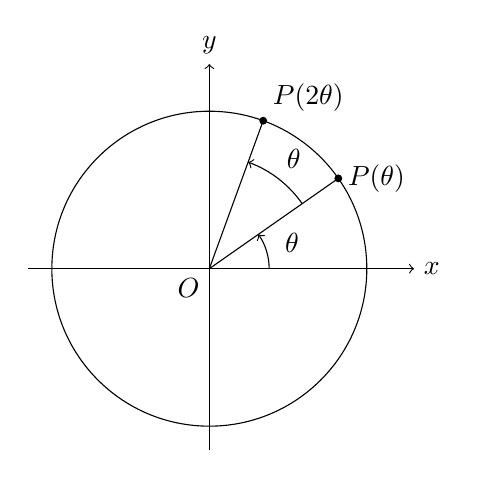
\begin{tikzpicture}[scale=2]
        \draw[->] (-1.15,0) -- (1.3,0) node[right] {$x$};
        \draw[->] (0,-1.15) -- (0,1.3) node[above] {$y$};
        \draw (0,0) circle (1);
        \node[below left] at (0,0) {$O$};
        \draw (0,0) -- (35:1);
        \draw (0,0) -- (70:1);
        \fill (35:1) circle (0.025) node[right] {$P(\theta)$};
        \fill (70:1) circle (0.025) node[above right] {$P(2\theta)$};
        \draw[->] (0.38,0) arc (0:35:0.38);
        \node at (17.5:0.55) {$\theta$};
        \draw[->] (35:0.72) arc (35:70:0.72);
        \node at (52.5:0.88) {$\theta$};
      \end{tikzpicture}
      \BookFigureCaption{単位円における角度の倍化}
    \end{center}

    先ほどの\bookterm{sequence}{数列}では,$a_n$は点$P(\theta_n)$の横座標である.
    回転後の横座標が
    \[
      \cos(2\theta_n)=2\cos^2\theta_n-1=2a_n^2-1
    \]
    となり,更新を満たす.初めの角度は
    \[
      \frac{\pi}{6}\ \longrightarrow\ \frac{\pi}{3}
      \ \longrightarrow\ \frac{2\pi}{3}
      \ \longrightarrow\ \frac{4\pi}{3}
    \]
    と変わり,横座標は
    \[
      \frac{\sqrt{3}}{2}\ \longrightarrow\ \frac12
      \ \longrightarrow\ -\frac12
      \ \longrightarrow\ -\frac12
    \]
    と変わる.最後の二点は異なるが横座標は同じであり,\bookterm{sequence}{数列}の値だけでは点の動きを捉えきれない.

    一定角の回転なら$\theta_{n+1}=\theta_n+\phi$だが,倍角では回す角度が毎回変わる.
    点の角度は$2\pi$ごとに読み替えてよい.$P(\theta)$と$P(\theta+\pi)$は倍角で同じ点へ移るため,円周全体の写像としても一定角の回転とは異なる.

    \,\sectionref{節：極形式と複素平面}の見方を使えば,この操作はさらに短く書ける.
    \[
      z_n=\cos\theta_n+i\sin\theta_n
    \]
    と置くと,\bookterm{de-moivre}{ド・モアブルの定理}より
    \[
      z_{n+1}=z_n^2,\qquad z_n=z_1^{\,2^{n-1}}
    \]
    となる.絶対値1の$z_n$を自身に掛け,角度をもう一度加えた.$a_n$はその実部である.

    \subsubsection{正接と傾き}\label{節：正接では直線の傾きを記録する}
    今度は
    \[
      a_1=\tan\frac{\pi}{12}=2-\sqrt{3},
      \quad
      a_{n+1}=\frac{2a_n}{1-a_n^2}
    \]
    を考える.右辺は$\tan$の倍角公式そのものである.したがって,
    \[
      a_n=\tan\left(2^{n-1}\frac{\pi}{12}\right)
    \]
    と予想できる.

    初項に一致し,帰納法の段階では
    \begin{align*}
      a_{n+1}
        &=\frac{2a_n}{1-a_n^2}\\
        &=\cfrac{2\tan\left(2^{n-1}\cfrac{\pi}{12}\right)}
                {1-\tan^2\left(2^{n-1}\cfrac{\pi}{12}\right)}\\
        &=\tan\left(2^n\frac{\pi}{12}\right)
    \end{align*}
    となる.分母が0にならないことは,角度から確かめる.

    $a_n=\tan\theta_n$は,原点と$P(\theta_n)$を通る直線の傾きである.
    倍角の動きを,今度は横座標でなく傾きで記録する.
    直線の向きは$\pi$ごとに同じになるが,縦向きでは傾きが定義できない.
    $a_n=\pm1$では$\cos(2\theta_n)=0$となり,この縦向きが分母$1-a_n^2=0$に対応する.
    なお,この例の角度は,$n\geq2$では
    \[
      \theta_n=\frac{2^{n-2}\pi}{6}
    \]
    である.$\displaystyle \theta_n=\frac{\pi}{2}+k\pi$となるには$2^{n-2}=3+6k$が必要だが,
    2の累乗は3の倍数でないので不可能である.初項でも傾きは定義できるため,全項が定義される.

  \subsubsection{角度の整数倍}\label{節：整数倍の公式へ}
    両例の方針は,
    \[
      a_n=\varphi(\theta_n),
      \quad
      \varphi(m\theta)=F_m(\varphi(\theta))
    \]
    を満たす関数と整数倍公式を探し,角度の更新を解くことである.

    また,ここで現れた多項式
    \[
      2x^2-1,
      \quad
      4x^3-3x
    \]
    も同じ族に属する.\bookterm{chebyshev}{チェビシェフ多項式}$T_m(x)$を
    \[
      T_m(\cos\theta)=\cos(m\theta)
    \]
    で定義すれば,
    \[
      T_0(x)=1,  T_1(x)=x,
    \]
    \[
      T_{m+1}(x)=2xT_m(x)-T_{m-1}(x)
    \]
    となる.例えば $T_2(x)=2x^2-1$ である.
    $T$の添字は角度の倍率なので,$\cos$の例は
    \[
      a_{n+1}=T_2(a_n),
      \quad
      a_n=T_{2^{n-1}}(a_1)
    \]
    と書ける.一回の更新では
    \[
      T_2(T_m(\cos\theta))=T_{2m}(\cos\theta)
    \]
    となり,添字は$2,4,8,\ldots$と進む.
    付録の\bookterm{chebyshev}{チェビシェフ多項式}では,この合成を一般の整数倍へ広げる.
